\documentclass[12pt]{article}
\usepackage{graphicx}
\usepackage{float}
\usepackage{wrapfig}
\usepackage[margin=3.0cm]{geometry}
\usepackage{hyperref}
\usepackage{amsmath}
\usepackage{fancyhdr}
\usepackage{tabularray}
\usepackage[absolute]{textpos}

\setlength{\TPHorizModule}{1cm}
\setlength{\TPVertModule}{1cm}


\begin{document}

\begin{textblock}{1}(1,1)
  
\includegraphics[width=2cm]{IIIT-Hyderabad-Logo.png}
  \label{fig:image}
\end{textblock}

\begin{center}
\textbf{\Large Matrix Models in Population Dynamics: Exploring Structure and Applications} \\

\vspace{1.5cc}
{ \sc Aryaman Bahl$^{1}$,Siddharth Agarwal$^{2}$, Sujal Keshri$^{3}$}\\

\vspace{0.3 cm}

{\small $^{1}$CND, International Institute of Information Technology, Hyderabad\\ $^{2}$CSE, International Institute of Information Technology, Hyderabad\\
$^{3}$ CSE, International Institute of Information Technology, Hyderabad\\}
\end{center}

\vspace{1.5cc}

\begin{abstract}
  \noindent  
This paper provides an overview of matrix models in population dynamics, focusing on population transitions, the Leslie matrix model, the SIR model, applications, and extensions. It discusses key findings and emphasizes the usefulness of matrix models in understanding and predicting population dynamics. The paper explores sensitivity analysis to examine the impact of birth rates, death rates, and migration on populations. It also addresses the effects of age-specific fertility and mortality rates on population growth and the prediction of population structure using stable age distribution. Extensions include stage-structured models, density-dependent models, and metapopulation models. The paper concludes by summarizing insights gained from matrix models and their importance in studying population dynamics.

\end{abstract}

\section{Introduction}
Population dynamics is a vital field of study with applications in ecology, demography, epidemiology, and conservation biology. This paper provides an introduction to the fundamental concepts and models used in population dynamics, focusing on matrix models. It explores the construction and interpretation of population transition matrices. The paper discusses the calculation of important population parameters and the prediction of future population sizes using matrix multiplication. Additionally, it examines the implications of the SIR model in the field of epidemiology. The practical applications of matrix models, their extensions, and alternative approaches are also discussed, offering valuable insights into the field of population dynamics.

\subsection{Matrix Models in Population Dynamics}
Matrix models provide a powerful framework for analyzing population dynamics. They allow us to capture the complex interactions between birth rates, death rates, immigration, and emigration. By representing these dynamics in a matrix format, we can systematically study how populations change over time.

\subsection{Construction and Interpretation of Population Transition Matrices}
One of the key components of matrix models is the population transition matrix. This matrix describes the probabilities of individuals transitioning from one state (e.g., age or stage class) to another over a specified time interval. The paper explores the construction of these matrices and delves into their interpretation within the context of population dynamics.

\subsection{Calculation of Important Population Parameters}
Matrix models enable us to calculate crucial population parameters, such as the net reproductive rate (Ro), which represents the average number of offspring produced by an individual throughout its lifetime. These parameters provide insights into population growth, stability, and potential for future change.

\subsection{Prediction of Future Population Sizes}
Using matrix multiplication, it becomes possible to predict future population sizes based on the initial population distribution and the population transition matrix. This predictive capability is valuable for assessing population trends and planning appropriate conservation or management strategies.

\subsection{Implications of the SIR Model in Epidemiology}
The paper also discusses the SIR (Susceptible-Infectious-Recovered) model, which is widely used in epidemiology to understand and control the spread of infectious diseases within populations. The SIR model incorporates concepts of population dynamics, disease transmission, and recovery, providing valuable insights for public health interventions.

\subsection{Practical Applications of Matrix Models}
The practical applications of matrix models in population dynamics are explored. Sensitivity analysis allows us to assess the impact of changes in birth rates, death rates, and migration on population dynamics. The effects of age-specific fertility and mortality rates on population growth can be investigated. Stable age distribution, a concept derived from matrix models, helps predict population structure and age composition.

\subsection{Extensions and Alternative Approaches}
Matrix models serve as a foundation for more complex population models. The paper discusses stage-structured models that account for different life stages, density-dependent models that consider population size effects, and metapopulation models that study interactions among multiple subpopulations. Furthermore, the role of stochasticity and uncertainty in population dynamics is examined. Alternative modeling approaches beyond matrix models are also considered.

\section{Matrix Models in Population Dynamics}

Matrix models are powerful tools used in population dynamics to study the dynamics of structured populations. In a matrix model, population characteristics, such as age, size, or stage, are organized into discrete classes. The population transition from one class to another is represented by a matrix, where each element represents the probability or rate of transition. These models allow for the analysis of population growth, age or stage structure, and the effects of vital rates (birth, death, and migration) on population dynamics. Matrix models provide insights into population stability, extinction risk, and the impacts of environmental changes. They are widely used in ecology, conservation biology, and demography to inform conservation strategies, wildlife management, and understanding population responses to environmental disturbances.
\subsection{Population Dynamics over time}
Population dynamics studies changes in population size and composition over time. Markov chains are useful for modeling population dynamics, representing transitions between different states or classes. Transition probabilities in the chain indicate the likelihood of moving between states. Markov chain models enable the analysis of population growth, stability, and the effects of factors on population structure. They aid in predicting future trends and understanding the impacts of interventions. Markov chains form the basis for complex models incorporating birth/death rates, migration, and environment. They support decision-making, policy formulation, and addressing population management challenges in ecology, epidemiology, economics, and social sciences.
\begin{figure}[H]
  \centering
  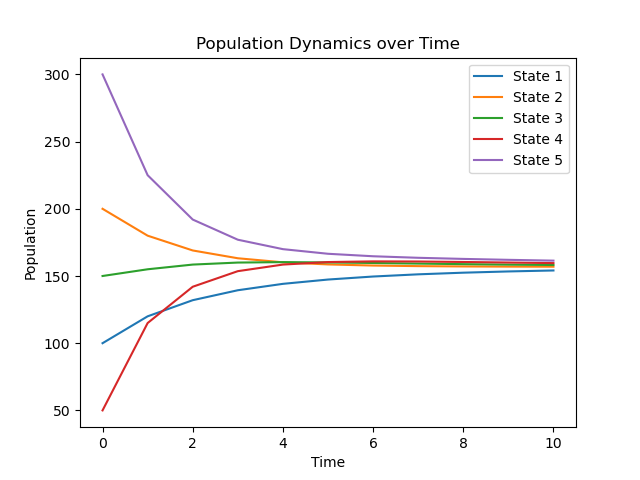
\includegraphics[width=0.4\textwidth]{Figure_3.png}
\end{figure}

\subsection{Population Growth varying with Time,Space,Stability graph}
\subsubsection{Time}
The rate of change in population size can be calculated by multiplying the population vector by the matrix. This gives a new vector that represents the population size at a later time.

\begin{equation}
\mathbf{x}(t + 1) = A \mathbf{x}(t)
\end{equation}
For example, let's say that the population vector is x=(100,200,300), and the matrix is A=(1.05,0.02,0.01). This means that the birth rate is 5 percent , the death rate is 2 percent, and the immigration rate is 1 percent.\\\\
If we multiply the population vector by the matrix, we get the new vector x(t+1)=(105,204,303). This means that the population size will increase to 105 in the next time period.\\\\
This is just a simple example, but it illustrates how population size can be modeled using linear algebra. This can be used to predict how population size will change over time, and to help policymakers make decisions about how to manage population growth.
Here are some additional points about how population size depends on time with respect to linear algebra:\\\\
The rate of population growth is not always constant. It can change over time due to factors such as war, famine, disease, and technological advances.\\\\
The population size of a species can also be affected by the population size of other species. For example, the population size of predators can affect the population size of prey.\\\\
Linear algebra can be used to model the interactions between different species, and to predict how these interactions will affect population sizes over time.
\begin{figure}[H]
  \centering
  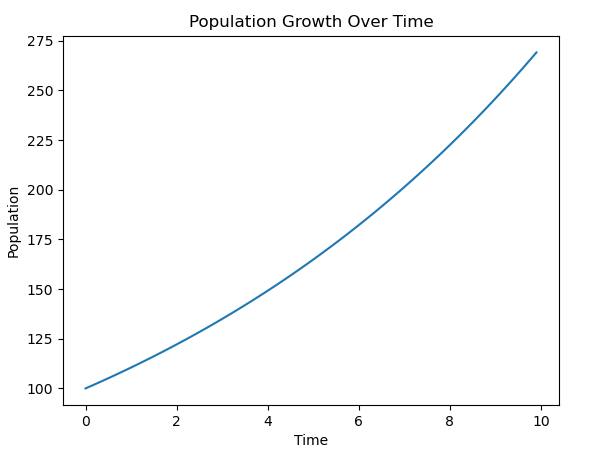
\includegraphics[width=0.4\textwidth]{timefianl.png}
\end{figure}
\subsubsection{Space}
Sure, here is a short note on how population size depends on space with respect to linear algebra:
In linear algebra, a vector can be used to represent a population. The vector's components can represent the population's size, density, and distribution in space. The population size can be calculated by taking the sum of the components of the vector. The population density can be calculated by dividing the population size by the area of the space. The population distribution can be calculated by finding the average value of the components of the vector.\\\\
The population size can depend on space in a number of ways. For example, the population size may be larger in areas with more resources, such as food and water. The population size may also be larger in areas with a more favorable climate. The population size may also be larger in areas with a shorter distance to other populations.\\\\
Linear algebra can be used to model the relationship between population size and space. This can be used to predict how population size will change over time, or to identify factors that influence population size.\\\\
Here are some examples of how linear algebra can be used to study population size:\\\\
A researcher can use linear algebra to model the relationship between population size and the availability of food. This could be used to predict how a population might change in size if there is a drought or a flood.\\\\
A conservationist can use linear algebra to model the relationship between population size and the amount of habitat available. This could be used to identify areas where conservation efforts are needed to protect a population from extinction.\\\\
A city planner can use linear algebra to model the relationship between population size and the availability of housing. This could be used to plan for future population growth and to ensure that there is enough housing available for everyone.
\begin{figure}[H]
  \centering
  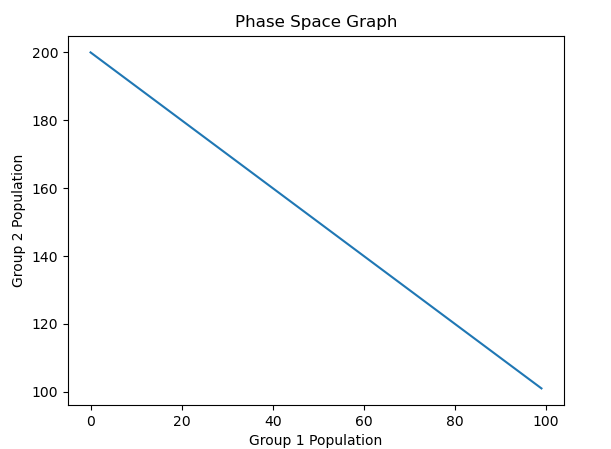
\includegraphics[width=0.4\textwidth]{spacefinal.png}
\end{figure}
\subsubsection{Stabilitiy}
Inaddition to diversity, population size can also affect stability through the concept of carrying capacity. Carrying capacity is the maximum population size that an environment can sustain over time. If a population exceeds its carrying capacity, it will begin to decline. This can happen due to a variety of factors, such as resource depletion or environmental degradation. Larger populations are more likely to exceed their carrying capacity than smaller populations, as they put more stress on the environment.\\\\
The relationship between population size and stability can be seen in a number of different contexts. For example, in ecology, it is known that larger populations are more likely to be stable than smaller populations. This is because larger populations have more genetic diversity, which can help them to adapt to changes in their environment. In economics, it is also known that larger economies are more stable than smaller economies. This is because larger economies have more diversified industries, which can help them to weather economic downturns.\\\\
Here are some additional examples of how population size can affect stability:\\\\
In a political system, a larger population can make it more difficult for one group to gain control and maintain power. This is because there are more people with different interests and opinions, which makes it more difficult for any one group to dominate.
In a business, a larger customer base can make the business more stable. This is because there are more people who are buying the company's products or services, which provides the company with a steady stream of income. In a community, a larger population can make it more difficult for crime to occur. This is because there are more people who are watching out for each other and reporting crimes to the police.\\\\
\begin{figure}[H]
  \centering
  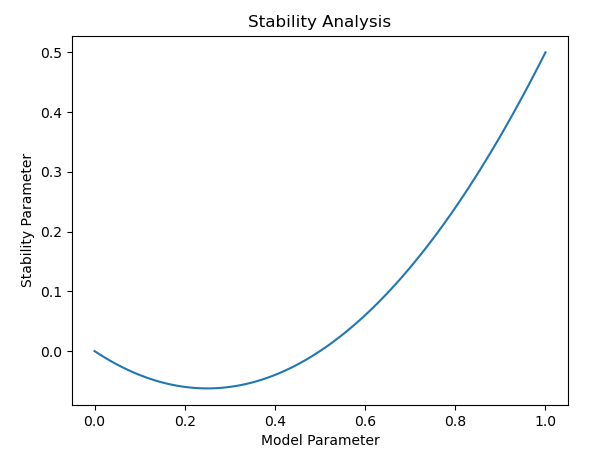
\includegraphics[width=0.5\textwidth]{stabilityfinal.png}
\end{figure}
\section{Markov Chains} 
A Markov chain or Markov process is a stochastic model describing a sequence of possible events in which the probability of each event depends only on the state attained in the previous event.Informally, this may be thought of as, "What happens next depends only on the state of affairs now." A countably infinite sequence, in which the chain moves state at discrete time steps, gives a \href{https://en.wikipedia.org/wiki/Discrete-time_Markov_chain}{discrete-time Markov chain}(DTMC). A continuous-time process is called a \href{https://en.wikipedia.org/wiki/Continuous-time_Markov_chain}{continuous-time Markov chain} (CTMC). It is named after the Russian mathematician \href{https://en.wikipedia.org/wiki/Andrey_Markov}{Andrey Markov}.

\subsection{Types Of Markov Chain}
The system's state space and time parameter index need to be specified. The following table gives an overview of the different instances of Markov processes for different levels of state space generality and for discrete time v. continuous time:\\\\
\begin{tabularx}{0.8\textwidth}{| c | c | c |}
    \hline
    \textbf{} & \textbf{Countable state space} & \textbf{Continuous or general state space} \\
    \hline
    Discrete-time & (discrete-time) Markov chain on a countable or finite state space & Markov chain on a measurable state space \\
    \hline
    Continuous-time & Continuous-time Markov process or Markov jump process & Any continuous stochastic process with the Markov property \\
    \hline
\end{tabularx}

\subsection{Prerequisites for Markov Chain}

\subsubsection{Stochastic process}
A stochastic (or random) process is a sequence of experiments for which the outcome at any stage depends on chance. In a simple model, there are a finite number of possible outcomes, referred to as states, and the process occurs in discrete time.\\\\
Let $S$ denote the set of states. Then, the stochastic process is a sequence $s_0, s_1, s_2, \ldots$, where all $s_n \in S$ depend on chance.

\subsubsection{Bernoulli scheme}
A Bernoulli scheme is a sequence of independent random events. In the sequence $s_0, s_1, s_2, \ldots$, any outcome $s_n$ is independent of the others.\\\\
For any integer $n \geq 0$, we have a probability distribution $p(n)$ on $S$. This means that each state $s \in S$ is assigned a value $p(n)_s \geq 0$ such that $\sum_{s \in S} p(n)_s = 1$. Then, the probability of the event $s_n = s$ is $p(n)_s$.\\
The Bernoulli scheme is called stationary if the
probability distributions $p
(n) $do not depend on n.

\subsection{Markov Chain}
A Markov chain is a stochastic process with discrete time such that the probability of the next outcome depends only on the previous outcome.\\\\
Let $S = \{1, 2, \ldots, k\}$. The Markov chain is determined by transition probabilities $p(t)_{ij}$, $1 \leq i, j \leq k$, $t \geq 0$, and by the initial probability distribution $q_i$, $1 \leq i \leq k$.
Here, $q_i$ is the probability of the event $s_0 = i$, and $p(t)_{ij}$ is the conditional probability of the event $s_{t+1} = j$ provided that $s_t = i$. By construction, we have $p(t)_{ij}, q_i \geq 0$, $\sum_i q_i = 1$, and $\sum_j p(t)_{ij} = 1$.\\\\
We shall assume that the Markov chain is time-independent, i.e., transition probabilities do not depend on time: $p_{t_{ij}} = p_{ij}$. Then, a Markov chain on $S = \{1, 2, \ldots, k\}$ is determined by a probability vector $x_0 = (q_1, q_2, \ldots, q_k) \in \mathbb{R}^k$ and a $k \times k$ transition matrix $P = (p_{ij})$. The entries in each row of $P$ add up to 1.\\\\
Let $s_0, s_1, s_2, \ldots$ be the Markov chain. Then the vector $x_0$ determines the probability distribution of the initial state $s_0$.
\subsubsection{Visualization:} 
We can visualize Markov chains with directed graphs.
\begin{itemize}
    \item Vertices of the graph represent the states (entries of a vector).
    \item Arrows of the graph represent the transitions and their probability.
    \item We can write the transition probabilities into a stochastic matrix $P$.
\end{itemize}\\\\
\begin{figure}[H]
  \centering
  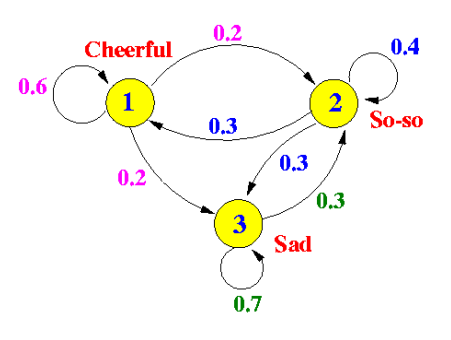
\includegraphics[width=0.6\textwidth]{cheerful.png}
\end{figure}


\subsubsection{Taking Example of a Random Walk:}
\begin{figure}[H]
  \centering
  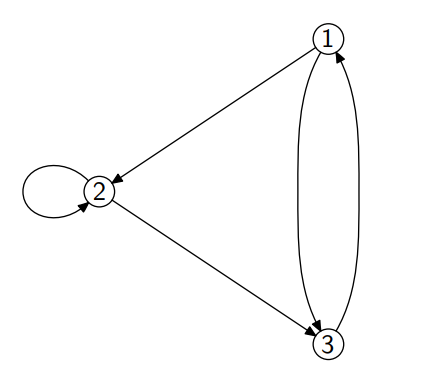
\includegraphics[width=0.4\textwidth]{random walk.png}
\end{figure}
\begin{equation}
Transition Matrix = 
\[
\begin{pmatrix}
0 & 0.5 & 0.5 \\
0 & 0.5 & 0.5 \\
1 & 0 & 0 \\
\end{pmatrix}
\]
\end{equation}

\subsubsection{Very primitive weather model:}
Two states: "sunny" (1) and "rainy" (2).
Transition matrix: P =
\begin{bmatrix}
0.9 & 0.1 \\
0.5 & 0.5 \\
\end{bmatrix}
.
Suppose that $\mathbf{x}_0 = (1, 0)$ (sunny weather initially).\\\\
Make a long-term weather prediction. The probability distribution of weather for day $n$ is given by the vector $\mathbf{x}_n^\intercal = Q^n \mathbf{x}_0^\intercal$, where $Q = P^\intercal$.\\\\
To compute $Q^n$, we need to diagonalize the matrix
$Q =
\begin{pmatrix}
0.9 & 0.5 \\
0.1 & 0.5 \\
\end{pmatrix}$.
$\text{det}(Q - \lambda I) =
\begin{vmatrix}
0.9 - \lambda & 0.5 \\
0.1 & 0.5 - \lambda \\
\end{vmatrix} =
\lambda^2 - 1.4\lambda + 0.4 = (\lambda - 1)(\lambda - 0.4)$.
Two eigenvalues: $\lambda_1 = 1$, $\lambda_2 = 0.4$.
$(Q - I)\mathbf{v} = 0 \iff
\begin{pmatrix}
-0.1 & 0.5 \\
0.1 & -0.5 \\
\end{pmatrix} \begin{pmatrix}
x \\
y \\
\end{pmatrix} =
\begin{pmatrix}
0 \\
0 \\
\end{pmatrix} \iff (x, y) = t(5, 1), t \in \mathbb{R}$.
$(Q - 0.4I)\mathbf{v} = 0 \iff
\begin{pmatrix}
0.5 & 0.5 \\
0.1 & 0.1 \\
\end{pmatrix} \begin{pmatrix}
x \\
y \\
\end{pmatrix} =
\begin{pmatrix}
0 \\
0 \\
\end{pmatrix} \iff (x, y) = t(-1, 1), t \in \mathbb{R}$.
$\mathbf{v}_1 = \begin{pmatrix}
5 \\
1 \\
\end{pmatrix}^\intercal$ and $\mathbf{v}_2 = \begin{pmatrix}
-1 \\
1 \\
\end{pmatrix}^\intercal$ are eigenvectors of $Q$ belonging to eigenvalues 1 and 0.4, respectively.
$\mathbf{x}_0^\intercal = \alpha \mathbf{v}_1 + \beta \mathbf{v}_2 \iff
\begin{cases}
5\alpha - \beta = 1 \\
\alpha + \beta = 0 \\
\end{cases} \iff
\begin{cases}
\alpha = \frac{1}{6} \\
\beta = -\frac{1}{6} \\
\end{cases}$
Now $\mathbf{x}_n^\intercal = Q^n \mathbf{x}_0^\intercal = Q^n(\alpha \mathbf{v}_1 + \beta \mathbf{v}_2) = \alpha \mathbf{v}_1 + (0.4)^n \beta \mathbf{v}_2$, which converges to the vector $\alpha \mathbf{v}_1 = \begin{pmatrix}
\frac{5}{6} \\
\frac{1}{6} \\
\end{pmatrix}^\intercal$ as $n \to \infty$.
The vector $\mathbf{x}_\infty = \begin{pmatrix}
\frac{5}{6} \\
\frac{1}{6} \\
\end{pmatrix}$ gives the limit distribution. Also, it is a steady-state vector.

\subsubsection{Representation of population growth using Markovs chain}
Note we will be using various python libraries like Pandas, Numpy, MatPlotLib etc. for manipulating data and plotting graphs and images. All the code related to this discussion here can be found in this \href{https://github.com/ABiiitH/LA_Project_Population.git}{Git Repo}.
\begin{figure}[H]
  \centering
  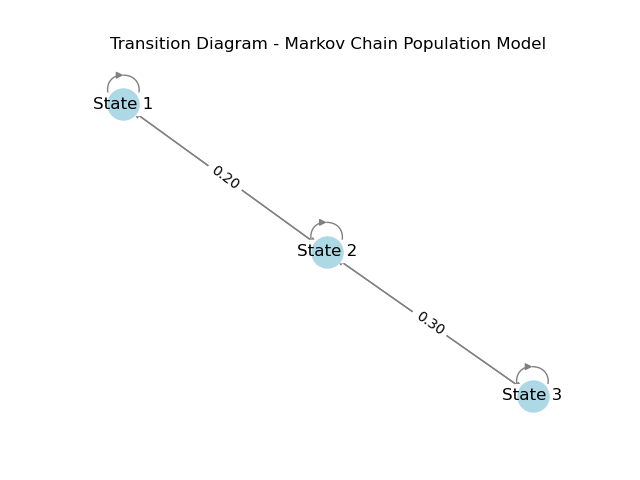
\includegraphics[width=0.6\textwidth]{Figure_2.png}
\end{figure}

\section{Leisle Model}
The Leslie matrix is a discrete, age-structured model of population growth that is very popular in population ecology named after \href{https://en.wikipedia.org/wiki/Patrick_Holt_Leslie}{Patrick H. Leslie} .The Leslie matrix (also called the Leslie model) is one of the most well-known ways to describe the growth of populations (and their projected age distribution), in which a population is closed to migration, growing in an unlimited environment, and where only one sex, usually the female, is considered. The Leslie matrix is used in ecology to model the changes in a population of organisms over a period of time. In a Leslie model, the population is divided into groups based on age classes.The Leslie matrix is a square matrix with the same number of rows and columns as the population vector has elements. The (i,j)th cell in the matrix indicates how many individuals will be in the age class i at the next time step for each individual in stage j. At each time step, the population vector is multiplied by the Leslie matrix to generate the population vector for the subsequent time step.
\subsection{Leslie Matrix Construction}
To build a matrix, the following information must be known from the population:
\begin{itemize}
\item $n_{x}$: the count of individuals ($n$) of each age class $x$
\item $s_{x}$: the fraction of individuals that survives from age class $x$ to age class $x+1$
\item $f_{x}$: fecundity, the per capita average number of female offspring reaching $n_{0}$ born from mother of age class $x$. More precisely, it can be viewed as the number of offspring produced at the next age class $x+1$ weighted by the probability of reaching the next age class. Therefore, $f_x = s_xb_{x+1}$
\end{itemize}
From the observations that $n_{0}$ at time $t+1$ is simply the sum of all offspring born from the previous time step and that the organisms surviving to time $t+1$ are the organisms at time $t$ surviving at probability $s_{x}$, one gets $n_{x+1} = s_xn_x$. This implies the following matrix representation:
\begin{figure}[H]
  \centering
  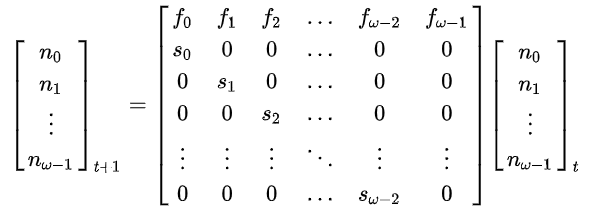
\includegraphics[width=0.6\textwidth]{leslie model.png}
\end{figure}
where $\omega$ is the maximum age attainable in the population.\\\\
The Leslie model is very similar to a discrete-time Markov chain. The main difference is that in a Markov model, one would have $f_x + s_x = 1$ for each $x$, while the Leslie model may have these sums greater or less than 1.
\subsection{
Determining Stable Age Distribution}
Whether we are dealing with age classes or ages, individuals are grouped into discrete classes that are of equal duration for modeling purposes. A typical life cycle of a population with age-class structure is:
\begin{figure}[H]
  \centering
  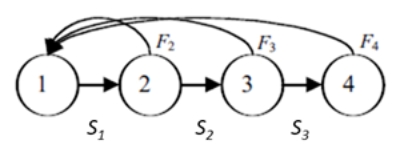
\includegraphics[width=0.6\textwidth]{birthtodeath.png}
\end{figure}
The life cycle of a population with age-class structure is depicted using circles to represent different age classes. In this example, we focus on a population with four age classes. The horizontal arrows connecting the circles represent survival probabilities (Sx), indicating the likelihood of an individual at age x surviving to age x + 1. Notably, there is no arrow from age four to age five, signifying a 0 probability of surviving to the fifth age class. The curved arrows at the top represent births, with all arrows leading to age 1 as newborns enter the first age class. The diagram illustrates that individuals aged 2, 3, and 4 are capable of reproduction, while those in age class 1 do not reproduce. If only age class 4 individuals reproduced, the diagram would require modification.
\begin{figure}[H]
  \centering
  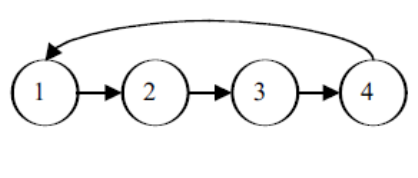
\includegraphics[width=0.6\textwidth]{modifiedbirthtodeath.png}
\end{figure}
\subsection{ Population Projection Matrix}
For example, with 3 age classes (ages 0-2, females only) the Leslie matrix would take the form:\\\\
\begin{equation}
A= 
\begin{pmatrix}
F_{0} & F_{1} & F_{2} \\
S_{0} & 0 & 0 \\
0 & S_{1} & 0 \\
\end{pmatrix}

\end{equation}
\(F_x\) = age specific fecundity\\
S_x = age specific survival rate\\\\
Leslie Matrix (A) replaces l in the shift from a simple exponential growth curve to an age-structured population growth model (note, this is still exponential after shifting)
N_{t+1} = N_t \lambda^l, \quad N_t = N_0 \lambda^t
sfiavdfwbge






\end{document}
